

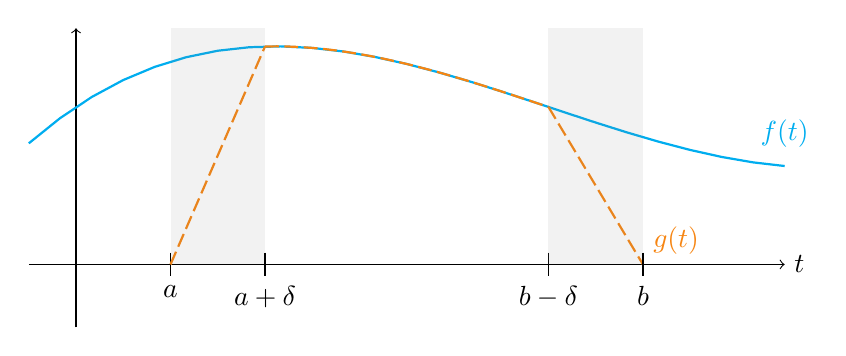
\begin{tikzpicture}[xscale=6,yscale=2]
    %* Draw axes
    \draw[->] (-0.1,0) -- (1.5,0) node[right] {$t$};  % går fra -0.3 til 1.5 på X aksen
    \draw[->] (0,-0.4) -- (0,1.5); %node[above] {$y$};  % går fra -0.4 til 1.5 på Y aksen
    
    %* Plot polynomial function
    \draw[cyan, thick, domain = -0.1:1.5] plot (\x, {(\x-1)^3 - (\x-1) + 1}) node[above, yshift=1mm] {$f(t)$};


    %* Draw labeled marks on the x-axis
    \foreach \x in { 0.2 }{
        \draw (\x,0.075) -- (\x,-0.075) node[below] {$a$}; % Lengden på linjen først
        %\draw[dashed] (\x,0) -- (\x,1.5);
        \draw[BurntOrange, dash pattern={on 5pt off 2pt}, thick] (\x,0) -- (0.4,{(0.4-1)^3 - (0.4-1) + 1});  % end value is the function value
    }

    %* Shade area between the points above and below
    \fill[gray, opacity=0.1] (0.2,0) -- (0.2,1.5) -- (0.4,1.5) -- (0.4,0) -- cycle;
    %\draw[pattern={north east lines},pattern color=gray] (0.2,0) rectangle +(0.2,1.5);

    %* Draw labeled marks on the x-axis
    \foreach \x in { 0.4 }{
        \draw (\x,0.075) -- (\x,-0.075) node[below] {$a+\delta$}; % Lengden på linjen først
        %\draw[dashed] (\x,0) -- (\x,1.5);
    }

    %* draw the middle parts of the approximating function g  —————— MIDDLE ——————
    %\draw[red, thick, dashed, domain=0.4:1] plot (\x, {(\x-1)^3 - (\x-1) + 1}) node[anchor=south east, yshift=2mm] {$g(t)$};
    %\draw[BurntOrange, thick, dashed, domain=0.4:1] plot (\x, {(\x-1)^3 - (\x-1) + 1});
    \draw[BurntOrange, thick, dash pattern={on 5pt off 2pt}, domain=0.4:1] plot (\x, {(\x-1)^3 - (\x-1) + 1});
    

    %* Draw labeled marks on the x-axis
    \foreach \x in { 1 }{
        \draw (\x,0.075) -- (\x,-0.075) node[below] {$b-\delta$}; % Lengden på linjen først
        %\draw[dashed] (\x,0) -- (\x,1.5);
        \draw[BurntOrange, dash pattern={on 5pt off 2pt}, thick] (\x,{(\x-1)^3 - (\x-1) + 1}) -- (1.2,0) node[anchor=south west, yshift=0mm] {$g(t)$};  % end value is the function value
    }

    %* Shade area between the points above and below
    \fill[gray, opacity=0.1] (1,0) -- (1,1.5) -- (1.2,1.5) -- (1.2,0) -- cycle;

    %* Draw labeled marks on the x-axis
    \foreach \x in { 1.2 }{
        \draw (\x,0.075) -- (\x,-0.075) node[below] {$b$};
        %\draw[dashed] (\x,0) -- (\x,1.5);
    }

    %\fill[gray, opacity=0.3] (0.2,0) -- (0.2,{(0.2-1)^3 - (0.2-1) + 1}) -- (0.4,{(0.4-1)^3 - (0.4-1) + 1}) -- (0.4,0) -- cycle;

\end{tikzpicture}


\mycomment{  %! Whole middle fill with dotted lines
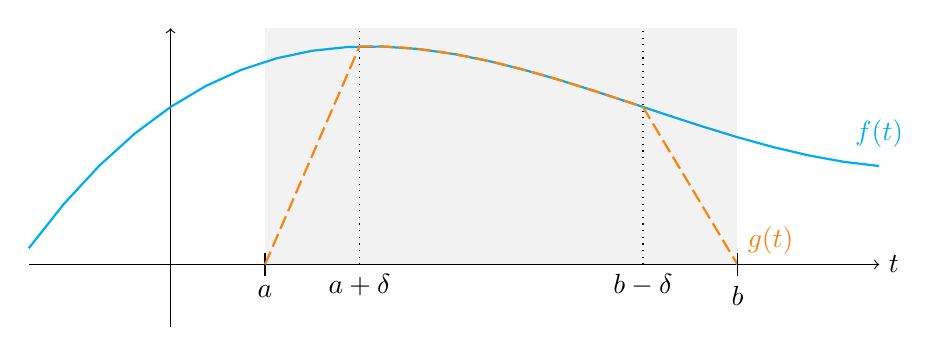
\begin{tikzpicture}[xscale=6,yscale=2]
    %* Draw axes
    \draw[->] (-0.3,0) -- (1.5,0) node[right] {$t$};  % går fra -0.3 til 1.5 på X aksen
    \draw[->] (0,-0.4) -- (0,1.5); %node[above] {$y$};  % går fra -0.4 til 1.5 på Y aksen
    
    %* Plot polynomial function
    \draw[cyan, thick, domain=-0.3:1.5] plot (\x, {(\x-1)^3 - (\x-1) + 1}) node[above, yshift=1mm] {$f(t)$};
    %* Shade area 
    \fill[gray, opacity=0.1] (0.2,0) -- (0.2,1.5) -- (1.2,1.5) -- (1.2,0) -- cycle;

    %* Draw labeled marks on the x-axis
    \foreach \x in { 0.2 }{
        \draw (\x,0.075) -- (\x,-0.075) node[below] {$a$}; % Lengden på linjen først
        %\draw[dashed] (\x,0) -- (\x,1.5);
        \draw[BurntOrange, dash pattern={on 5pt off 2pt}, thick] (\x,0) -- (0.4,{(0.4-1)^3 - (0.4-1) + 1});  % end value is the function value
    }

    %* Draw labeled marks on the x-axis
    \foreach \x in { 0.4 }{
        \draw (\x,0) -- (\x,-0.001) node[below] {$a+\delta$}; % Lengden på linjen først
        \draw[dotted] (\x,0) -- (\x,1.5);
    }

    %* draw the middle parts of the approximating function g  —————— MIDDLE ——————
    %\draw[red, thick, dashed, domain=0.4:1] plot (\x, {(\x-1)^3 - (\x-1) + 1}) node[anchor=south east, yshift=2mm] {$g(t)$};
    %\draw[BurntOrange, thick, dashed, domain=0.4:1] plot (\x, {(\x-1)^3 - (\x-1) + 1});
    \draw[BurntOrange, thick, dash pattern={on 5pt off 2pt}, domain=0.4:1] plot (\x, {(\x-1)^3 - (\x-1) + 1});
    

    %* Draw labeled marks on the x-axis
    \foreach \x in { 1 }{
        \draw (\x,0) -- (\x,-0.001) node[below] {$b-\delta$}; % Lengden på linjen først
        \draw[dotted] (\x,0) -- (\x,1.5);
        \draw[BurntOrange, dash pattern={on 5pt off 2pt}, thick] (\x,{(\x-1)^3 - (\x-1) + 1}) -- (1.2,0) node[anchor=south west, yshift=0mm] {$g(t)$};  % end value is the function value
    }


    %* Draw labeled marks on the x-axis
    \foreach \x in { 1.2 }{
        \draw (\x,0.075) -- (\x,-0.075) node[below] {$b$};
        %\draw[dashed] (\x,0) -- (\x,1.5);
    }

    %\fill[gray, opacity=0.3] (0.2,0) -- (0.2,{(0.2-1)^3 - (0.2-1) + 1}) -- (0.4,{(0.4-1)^3 - (0.4-1) + 1}) -- (0.4,0) -- cycle;

\end{tikzpicture}
}

\mycomment{  %! Whole middle fill with dashed lines
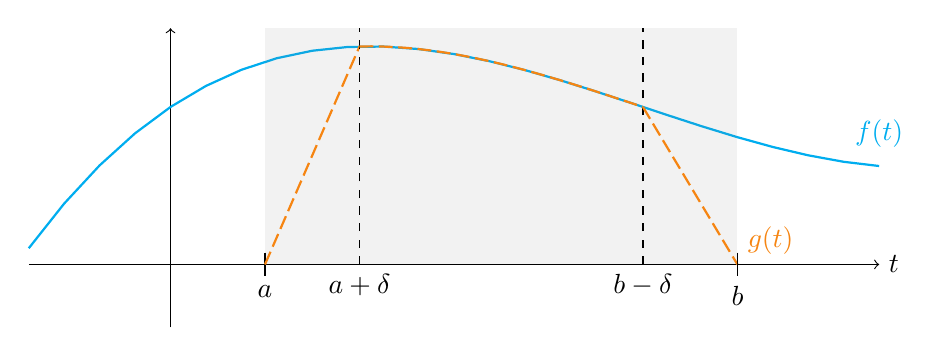
\begin{tikzpicture}[xscale=6,yscale=2]
    %* Draw axes
    \draw[->] (-0.3,0) -- (1.5,0) node[right] {$t$};  % går fra -0.3 til 1.5 på X aksen
    \draw[->] (0,-0.4) -- (0,1.5); %node[above] {$y$};  % går fra -0.4 til 1.5 på Y aksen
    
    %* Plot polynomial function
    \draw[cyan, thick, domain=-0.3:1.5] plot (\x, {(\x-1)^3 - (\x-1) + 1}) node[above, yshift=1mm] {$f(t)$};
    %* Shade area 
    \fill[gray, opacity=0.1] (0.2,0) -- (0.2,1.5) -- (1.2,1.5) -- (1.2,0) -- cycle;

    %* Draw labeled marks on the x-axis
    \foreach \x in { 0.2 }{
        \draw (\x,0.075) -- (\x,-0.075) node[below] {$a$}; % Lengden på linjen først
        %\draw[dashed] (\x,0) -- (\x,1.5);
        \draw[BurntOrange, dash pattern={on 5pt off 2pt}, thick] (\x,0) -- (0.4,{(0.4-1)^3 - (0.4-1) + 1});  % end value is the function value
    }

    %* Draw labeled marks on the x-axis
    \foreach \x in { 0.4 }{
        \draw (\x,0) -- (\x,-0.001) node[below] {$a+\delta$}; % Lengden på linjen først
        \draw[dashed] (\x,0) -- (\x,1.5);
    }

    %* draw the middle parts of the approximating function g  —————— MIDDLE ——————
    %\draw[red, thick, dashed, domain=0.4:1] plot (\x, {(\x-1)^3 - (\x-1) + 1}) node[anchor=south east, yshift=2mm] {$g(t)$};
    %\draw[BurntOrange, thick, dashed, domain=0.4:1] plot (\x, {(\x-1)^3 - (\x-1) + 1});
    \draw[BurntOrange, thick, dash pattern={on 5pt off 2pt}, domain=0.4:1] plot (\x, {(\x-1)^3 - (\x-1) + 1});
    

    %* Draw labeled marks on the x-axis
    \foreach \x in { 1 }{
        \draw (\x,0) -- (\x,-0.001) node[below] {$b-\delta$}; % Lengden på linjen først
        \draw[dashed] (\x,0) -- (\x,1.5);
        \draw[BurntOrange, dash pattern={on 5pt off 2pt}, thick] (\x,{(\x-1)^3 - (\x-1) + 1}) -- (1.2,0) node[anchor=south west, yshift=0mm] {$g(t)$};  % end value is the function value
    }


    %* Draw labeled marks on the x-axis
    \foreach \x in { 1.2 }{
        \draw (\x,0.075) -- (\x,-0.075) node[below] {$b$};
        %\draw[dashed] (\x,0) -- (\x,1.5);
    }

    %\fill[gray, opacity=0.3] (0.2,0) -- (0.2,{(0.2-1)^3 - (0.2-1) + 1}) -- (0.4,{(0.4-1)^3 - (0.4-1) + 1}) -- (0.4,0) -- cycle;

\end{tikzpicture}
}


\mycomment{  %! Whole middle fill with dashed lines and solid lines at the end
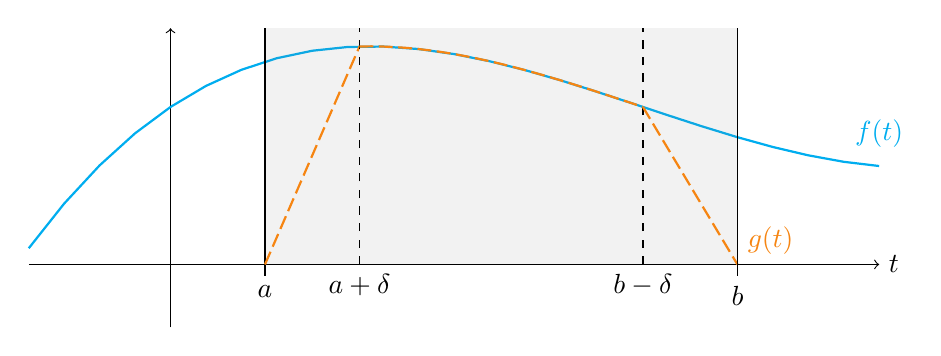
\begin{tikzpicture}[xscale=6,yscale=2]
    %* Draw axes
    \draw[->] (-0.3,0) -- (1.5,0) node[right] {$t$};  % går fra -0.3 til 1.5 på X aksen
    \draw[->] (0,-0.4) -- (0,1.5); %node[above] {$y$};  % går fra -0.4 til 1.5 på Y aksen
    
    %* Plot polynomial function
    \draw[cyan, thick, domain=-0.3:1.5] plot (\x, {(\x-1)^3 - (\x-1) + 1}) node[above, yshift=1mm] {$f(t)$};
    %* Shade area 
    \fill[gray, opacity=0.1] (0.2,0) -- (0.2,1.5) -- (1.2,1.5) -- (1.2,0) -- cycle;

    %* Draw labeled marks on the x-axis
    \foreach \x in { 0.2 }{
        \draw (\x,0.075) -- (\x,-0.075) node[below] {$a$}; % Lengden på linjen først
        \draw(\x,0) -- (\x,1.5);
        \draw[BurntOrange, dash pattern={on 5pt off 2pt}, thick] (\x,0) -- (0.4,{(0.4-1)^3 - (0.4-1) + 1});  % end value is the function value
    }

    %* Draw labeled marks on the x-axis
    \foreach \x in { 0.4 }{
        \draw (\x,0) -- (\x,-0.001) node[below] {$a+\delta$}; % Lengden på linjen først
        \draw [dashed] (\x,0) -- (\x,1.5);
    }

    %* draw the middle parts of the approximating function g  —————— MIDDLE ——————
    %\draw[red, thick, dashed, domain=0.4:1] plot (\x, {(\x-1)^3 - (\x-1) + 1}) node[anchor=south east, yshift=2mm] {$g(t)$};
    %\draw[BurntOrange, thick, dashed, domain=0.4:1] plot (\x, {(\x-1)^3 - (\x-1) + 1});
    \draw[BurntOrange, thick, dash pattern={on 5pt off 2pt}, domain=0.4:1] plot (\x, {(\x-1)^3 - (\x-1) + 1});
    

    %* Draw labeled marks on the x-axis
    \foreach \x in { 1 }{
        \draw (\x,0) -- (\x,-0.001) node[below] {$b-\delta$}; % Lengden på linjen først
        \draw [dashed] (\x,0) -- (\x,1.5);
        \draw[BurntOrange, dash pattern={on 5pt off 2pt}, thick] (\x,{(\x-1)^3 - (\x-1) + 1}) -- (1.2,0) node[anchor=south west, yshift=0mm] {$g(t)$};  % end value is the function value
    }


    %* Draw labeled marks on the x-axis
    \foreach \x in { 1.2 }{
        \draw (\x,0.075) -- (\x,-0.075) node[below] {$b$};
        \draw (\x,0) -- (\x,1.5);
    }

    %\fill[gray, opacity=0.3] (0.2,0) -- (0.2,{(0.2-1)^3 - (0.2-1) + 1}) -- (0.4,{(0.4-1)^3 - (0.4-1) + 1}) -- (0.4,0) -- cycle;

\end{tikzpicture}
}